\section{Algoritme til detektering af gang og løb}\label{sec:algogangloeb}
\textit{Dette afsnit omhandler design, implementering og test af algoritmerne til detektering af aktiviteterne gang og løb.} 

\subsubsection{Design} \label{design_algo_g_l}
Algoritmen designes til at benytte accelerometerets data i forhold til \appref{pilot}. Dette design fremgår på \figref{fig:design_algoritme_gang_loeb}.
\begin{figure}[H]
	\centering
	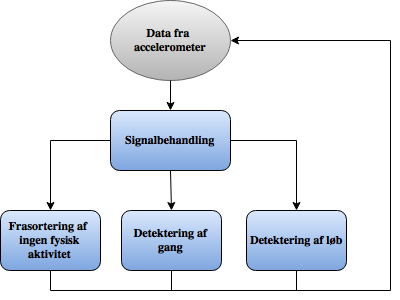
\includegraphics[scale=0.5]{figures/cDesign/design_algoritme_gang_loeb.png}
	\caption{På figuren ses et overordnet flowchart af algoritmen til detektering af ingen fysisk aktivitet, gang eller løb.}
	\label{fig:design_algoritme_gang_loeb}
\end{figure}\vspace{-0.25cm}
Algoritmen skal benytte accelerometerets data til at detektere, hvorvidt brugeren ikke udfører fysisk aktivitet, går eller løber. Før denne detektering skal accelerometeres data signalbehandles for afslutningsvis at kunne benytte tærskelværdier til at detektere, hvilken aktivitet der udføres. Signalbehandlingen indebærer filtrering, dividering, kvadrering og moving average filtrering. Denne type signalbehandling er illustreret på \figref{fig:algoritme_behandling}.
\begin{figure}[H]
	\centering
	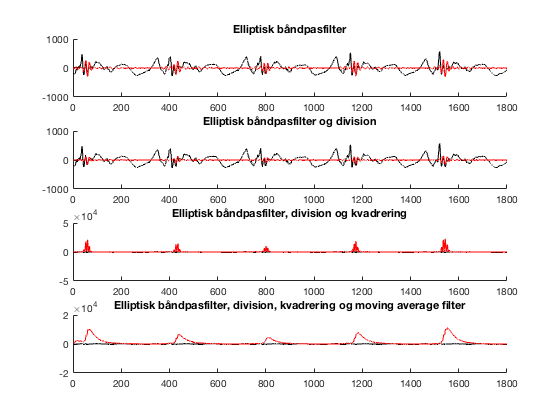
\includegraphics[width=1\textwidth]{figures/cDesign/signalbehandling_psoc.png}
	\caption{På figuren ses effekten af de fire typer af signalbehandling som udføres i algoritmen. Signalbehandlingen er illustreret på et råt signal fra accelerometerets y-akse under løb. Den sorte kurve er det rå signal, og den røde er det behandlede signal.}
	\label{fig:algoritme_behandling}
\end{figure}\vspace{-0.25cm}
Signalbehandlingen har til formål at tydeliggøre hælnedslag for derefter at kunne implementere tærskelværdier til adskillelse af de fysisk aktiviteter. \\
Første del af signalbehandlingen er en filtrering med et elliptisk båndpasfilter, som benyttes til at dæmpe støj. Dette skal være et fjerde ordens elliptisk båndpasfilter med et pasbånd fra 20~Hz til 50~Hz og med en dæmpning på 60~dB\fxnote{og 0.5 dB peak-to-peak ripples - frekvenserne for gang og løb lå mellem 25 og 45}. Båndpasfiltrets knækfrekvenser er valgt ud fra pilotforsøget i \appref{pilot}, hvorfra det vurderes at hælnedslag har en frekvens på 25~Hz til 45~Hz. Ved at benytte et båndpass filter bliver det ønskede signal i frekvensområdet 25-45~Hz bevaret, og andre frekvenser dæmpes.\\
Dernæst bliver signalet behandlet ved brug af en division, som har til formål at sænke amplituden af mindre peaks i signalet. Idet hælnedslaget besidder den største amplitude i signalet, bliver amplituden for hælnedslaget fortsat større end de mindre peaks. Efter signalet er blevet divideret, kvadreres signalet for at øge amplituden af de fremtrædende peaks i signalet. Dermed minimeres de mindre peaks, som ikke er relateret til hælnedslaget, og selve hælnedslaget forstærkes og tydeliggøres. Afslutningsvis filtreres signalet med et moving average filter, som udglatter signalet, hvorved små udslag ikke opfattes, og signalets hælnedslag vil fremstå som et enkelt peak.

Ovenstående signalbehandling bidrager til et signal med peaks, hvormed det er muligt at implementere tærskelværdier til adskillelse af gang og løb. Førend en værdi for denne tærskelværdi kan fastsættes skal dataet fra pilotforsøgets omregnes til ICens enhed for outputdata. ICens arbejdsområde er opgivet i bytes som følge af ICens 16~bits ADC arbejdsområde. Pilotforsøgets data skal derfor omregnes til bytes, idet data fra pilotforsøget er optaget med Shimmer3, som har enheden $m/s^{2}$. Derfor bliver pilotforsøgets data først omregnet til g ved at dividere med tyngdekraften. Herefter omregnes denne værdi i forhold til opløsningen for den 12~bits ADC, som findes i Shimmer3. For at gøre dette benyttes accelerometerets sensitivitet, som er 0,012~g/LSB. Data fra Shimmer3 skal divideres med accelerometerets sensitivitet. Outputet fra Shimmer3 og ICen besidder samme enhed, når data fra Shimmer3 er multipliceret med 16, som det fremgår af \eqref{eq:bitsammenhaeng}.
\begin{equation}
\frac{32~g~\cdot~2^{16}}{32~g~\cdot~2^{12}}~=~16
\label{eq:bitsammenhaeng}
\end{equation}
Data fra Shimmer3 skal derfor multipliceres med 16, hvilke medfører samme enhed for de to systemer. Det er derefter muligt at vurdere, hvilket tærskelværdier som kan benyttes til at detektere og adskille gang og løb.\\
De behandlede signaler fra pilotforsøget benyttes med henblik på fastsættelse af tærskelværdier. \Tabref{tab:individuel_taerskel} viser tærskelværdierne for de fire forsøgspersoner, hvoraf tærskelværdierne er vurderet til at dække samtlige peaks for det valgte tidsinterval. 
\begin{table}[H]
	\centering
	\begin{tabular}{ccc}
		\hline
		\rowcolor[HTML]{C0C0C0} 
		Forsøgsperson & Tærskelværdi for gang & Tærskelværdi for løb \\ \hline
		\rowcolor[HTML]{FFFFFF} 
		F1 & 50 & 1050 \\ \hline
		\rowcolor[HTML]{FFFFFF} 
		F2 & 55 & 500 \\ \hline
		\rowcolor[HTML]{FFFFFF} 
		F3 & 50 & 400 \\ \hline
		\rowcolor[HTML]{FFFFFF} 
		F4 & 150 & 1000 \\ \hline
	\end{tabular}
	\caption{I tabellen ses tærskelværdierne for forsøgspersonerne ved aktiviteterne gang og løb.}
	\label{tab:individuel_taerskel}
\end{table}\vspace{-0.25cm}
De individuelle tærskelværdier i \tabref{tab:individuel_taerskel} er fundet over et fem~sekunders vindue for hver forsøgsperson. Heraf antages det, at tærskelværdierne er repræsentative for den fysiske aktivitet, idet aktiviteten bliver udført ved konstant hastighed. Ydermere skal systemet være gældende for en stor population, hvormed en given tærskelværdierne for gang og løb skal være dækkende for alle forsøgspersoner. En samlet tærskelværdi, der er dækkende for samtlige forsøgspersoners data, ses i \tabref{tab:faelles_taerskel}.
\begin{table}[H]
	\centering
	\begin{tabular}{ccc}
		\hline
		\rowcolor[HTML]{C0C0C0} 
		Tærskelværdi for ingen fysisk aktivitet & Tærskelværdi for gang & Tærskelværdi for løb \\ \hline
		x~\textless~50 & 50 \textless~x~\textless~400 & x~$\geq$~400 \\ \hline
	\end{tabular}
	\caption{I tabellen ses de tærskelværdier, som for alle forsøgspersoner vil kunne detektere og adskille gang og løb.}
	\label{tab:faelles_taerskel}
\end{table}\vspace{-0.25cm}
Fastsættelsen af den fælles tærskelværdi bør sikre, at gang og løb er mulige at detektere samt adskille for forsøgspersonernes data. Behandlingen af data fra pilotforsøget påviser, at tærskelværdierne i \tabref{tab:faelles_taerskel} er dækkende for alle forsøgspersonerne, hvorfor disse bibeholdes.

\subsection{Implementering}
Implementeringen af algoritmen for detektering af gang og løb tager udgangspunkt i data fra pilotforsøget og de designmæssige aspekter, som er beskrevet i \secref{design_algo_g_l}. Algoritmen er designet og implementeret, som det ses på \figref{fig:basic_algo_g_l}.
\begin{figure}[H]
	\centering
	\includegraphics[scale=0.6]{figures/cDesign/Algoritme_g_l_basic.png}
	\caption{På figuren ses et flowchart over den implementerede C kode, som muliggør detektering af ingen fysisk aktivitet, gang og løb. Detektering af maksimalt peak er gældende for alle aktiviteterne. De markerede kasser indeholder yderligere C kode, som forklares uddybende efterfølgende.}
	\label{fig:basic_algo_g_l}
\end{figure}\vspace{-0.25cm}
Algoritmen henter low og high byte fra ICens outputdata, hvorefter de enkelte samples gennemgår en signalbehandling. Denne signalbehandling og den tilhørende C kode forklares yderligere i \figref{fig:signalbehandling_g_l}. Efter samples er blevet behandlet, bliver time counteren startet således, at denne tæller antallet af samples mellem bestemte if løkker i algoritmen. De behandlede samples gemmes i variabel 'Value[0]', hvortil den foregående behandlede sample bliver gemt i variabel 'Value[1]'. På denne måde kan algoritmen undersøge disse variabler i forhold til en tærskelværdi. \\
Efter den nye og foregående sample er placeret i separate variabler, er det muligt at benytte tærskelværdier til at detektere, hvorvidt der er gang, løb eller ingen aktivitet. Disse elementer af algoritmen forklares yderligere i \figref{fig:ingen_ak_pseudo}, \figref{fig:gang_pseudo} og \figref{fig:loeb_pseudo}. Tærskelværdierne for de pågældende fysiske aktiviteter er bestemt i \secref{design_algo_g_l}. \\ 
Yderligere bliver den maksimale peak bestemt, da denne værdi initialiserer, om det er gang eller løb i GUIen. Dette gøres ved at sammenligne, om den forrige sample er større end den nuværende. Hvis dette er tilfældet, betegnes den forrige sample som værende den maksimale peak værdi. %Når kurven derimod er faldende, vil detektering af maksimale peak ikke udføres.

Algoritmens signalbehandling involverer fire elementer; elliptisk filtrering, dividering, kvadrering og en moving average filtrering. Dette ses på \figref{fig:signalbehandling_g_l}.
\begin{figure}[H]
	\centering
	\includegraphics[scale=0.5]{figures/cDesign/Signalbehandling_gl_pesudo.png}
	\caption{På figuren ses flowchartet over algoritmens signalbehandling udført i C kode. Signalbehandlingen involverer elliptisk filtrering, dividering, kvadrering og en moving average filtrering.}
	\label{fig:signalbehandling_g_l}
\end{figure}\vspace{-0.25cm}
Efter datamodtagelse fra ICen bliver samples IIR filtreret ved hjælp af a og b koefficienter for et elliptisk filter. Efterfølgende retureneres de behandlede samples, hvormed disse er klar til næste del af signalbehandlingen. De pågældende a og b koefficienter bestemmes i MATLAB, hvor filterets knækfrekvenser og dæmpning benyttes til at bestemme det elliptiske filters koefficienter. Disse koefficienter skrives i C koden for algoritmen, således filtreringen udføres i henhold til det ønskede filter designet i MATLAB.\\
High byte for hver sample bliver herefter bitshiftet med 5, hvilket svarer til at dividere med 32\fxnote{2 opløftet i 5}. Derudover bliver hver sample med både high og low byte kvadreret. Afslutningsvis filtreres hver sample med et moving average filter, hvilket medfører en blødere kurve, som ses på \figref{fig:algoritme_behandling}.

Algoritmen er designet og implementeret således, at denne kan detektere, hvis brugeren ikke er fysisk aktiv. Denne del af algoritmen fremgår af \figref{fig:ingen_ak_pseudo}.
\begin{figure}[H]
	\centering
	\includegraphics[scale=0.6]{figures/cDesign/ingen_aktivitet_gl_pseudo.png}
	\caption{På figuren ses flowchartet over den algoritme, som er ansvarlig for detekteringen af ingen fysisk aktivitet. Algoritmen registrerer, at brugeren ikke er aktiv, når 'time\_count' er større end 1428~samples svarende til tre~sekunder.}
	\label{fig:ingen_ak_pseudo}
\end{figure}\vspace{-0.25cm}
Algoritmen detekterer, at brugeren ikke er fysisk aktiv, hvis time counteren opnår et antal samples, som er større end tre~sekunders sampling. Hvis dette er tilfældet, bliver de pågældende variabler nulstillet og tæller forfra.

Algoritmen benytter tærskelværdier til at bestemme, hvorvidt brugeren går eller løber. \Figref{fig:gang_pseudo} viser algoritmens opbygning i forhold til detektering af gang ved brug af tærskelværdier.
\begin{figure}[H]
	\centering
	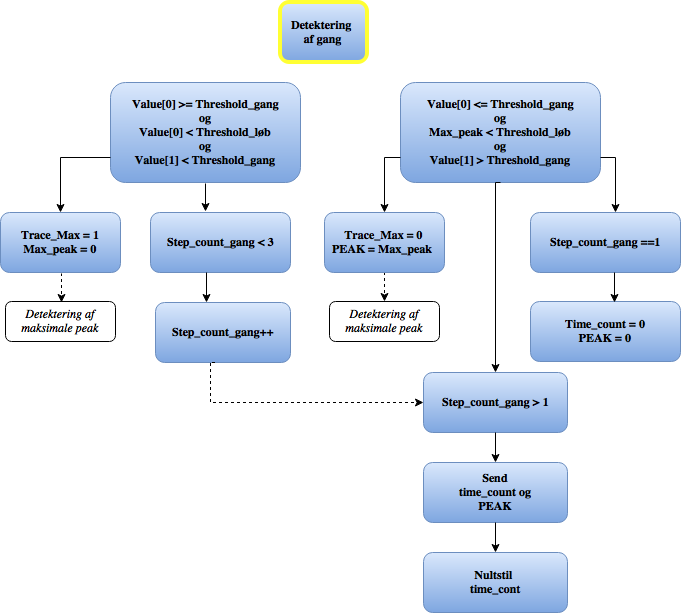
\includegraphics[scale=0.5]{figures/cDesign/gang_ckode_pseudo.png}
	\caption{På figuren ses et flowchart over algoritmen, der detekterer gang. Algoritmen benytter fastsatte tærskelværdier til denne detektering.}
	\label{fig:gang_pseudo}
\end{figure}\vspace{-0.25cm}
Til venstre på \figref{fig:gang_pseudo} ses den del, som er ansvarlig for optælling af skridt, hvortil den højre del visualiserer delen, som bestemmer varigheden mellem hælnedslag. Førend algoritmen kan tælle op på antal skridt for gang, skal amplituden for 'Value[0]' være i intervallet mellem tærskelværdierne for gang og løb. Yderligere skal den foregående sample 'Value[1]' have en værdi, der er lavere end tærskelværdien for gang. Hvis disse tre kriterier er opfyldt, indstilles Trace\_Max til at være lig 1. Dette tillader, at algoritmen begynder at finde den maksimale peak, som illustreret på \figref{fig:basic_algo_g_l}. Ydermere bliver Step\_count\_gang talt op, indtil denne variabel er maksimalt 3. \\
Højre del af \figref{fig:gang_pseudo} repræsenterer den del af algoritmen, som finder varigheden mellem hælnedslag og sender dette gennem BLE. Førend denne del af algoritmen bliver udført, skal 'Value[0]' være mindre end tærskelværdien for gang, og 'Value[1]' skal være over denne tærkselværdi. Yderligere skal det bestemte maksimale peak være mindre end tærskelværdien for løb. Hvis kriterierne opfyldes, bliver det maksimale peak gemt i PEAK, samt algoritmen indstilles således, at denne ikke længere finder et maksimalt peak. Yderligere er det gældende, at hvis der er detekteret et hælnedslag for gang, bliver henholdsvis time counteren og PEAK nulstillet. Det første detekterede maksimum peak fra signalet frasorteret for at sikre optimal optælling af varighed. \\
For at bestemme varigheden mellem hælnedslag skal antallet af hælnedslag for gang overstige værdien 1. Under disse omstændigheder bliver time\_count og PEAK bitshiftet for at muliggøre sammensætning af korrekt værdi, da resultatet gives i high byte og low byte. Disse værdier sendes afslutningsvist over BLE og time counteren nulstilles.

Algoritmen er desuden i stand til at detektere løb, hvilket også gøres ved brug af tærskelværdier, som det ses på \figref{fig:loeb_pseudo}.
\begin{figure}[H]
	\centering
	\includegraphics[scale=0.5]{figures/cDesign/loeb_ckode_pseudo.png}
	\caption{På figuren ses et flowchart over algoritmen, som detekterer løb. Algoritmen benytter fastsatte tærskelværdier til detektering af løb.}
	\label{fig:loeb_pseudo}
\end{figure}\vspace{-0.25cm}
Til venstre på \figref{fig:loeb_pseudo} ses delen, som er ansvarlig for optælling af skridt, hvortil den højre del visualiserer delen, som bestemmer varigheden mellem hælnedslag. Førend algoritmen kan tælle op på antal skridt for løb, skal amplituden for 'Value[0]' være større end tærskelværdien for løb. Yderligere skal den foregående sample 'Value[1]' have en størrelse, der er lavere end tærskelværdien for løb. Hvis disse to kriterier er opfyldt, indstilles Trace\_Max til at være lig 1. Dette tillader, at algoritmen begynder at finde den maksimale peak, som illustreret på \figref{fig:basic_algo_g_l}. Ydermere bliver 'Step\_count\_løb' talt op, indtil denne variabel er maksimalt 3. \\
Højre del af \figref{fig:loeb_pseudo} repræsenterer den del af algoritmen, som finder varigheden mellem hælnedslag og sender dette gennem BLE. Førend denne del af algoritmen bliver udført, skal 'Value[0]' være mindre end tærskelværdien for løb, og 'Value[1]' skal være over denne tærskelværdi. Hvis kriteriet opfyldes, bliver det maksimale peak gemt i 'PEAK' samt algoritmen indstilles således, at denne ikke længere finder et maksimalt peak. Yderligere er det gældende, at hvis der er detekteret ét hælnedslag for løb, bliver henholdsvis time counteren og 'PEAK' nulstillet. \\
For at bestemme varigheden mellem hælnedslag  skal antal hælnedslag for løb overstige værdien 1. Under disse omstændigheder bliver time\_count og PEAK bitshiftet for at muliggøre sammensætning af korrekt værdi, da resultatet gives i high byte og low byte. Disse værdier sendes afslutningsvist over BLE og time counteren nulstilles.

\subsection{Test}
Testen udføres på baggrund af de opstillede krav og tilhørende afvigelser opstillet i \secref{krav_algoritme}. Kravene beskriver, at algoritmen skal:
\begin{itemize}
	\item Behandle data fra accelerometret, således hælnedslag fremstår som et markant peak.
	\item Være i stand til at detektere gang og løb ved brug af tærskelværdier. Det accepteres ikke, at systemet ikke kan detektere og adskille gang og løb fra cykling.
\end{itemize}
Algoritmens funktioner testes individuelt og samlet. Dette gøres ved at indsende et simuleret signal, hvis funktion er at simulere gang, løb eller ingen aktivitet. Det simulerede signal er et absolut sinussignal med varierende amplitude. Amplituden for det simulerede signal afgør, hvorvidt signalet simulerer gang, løb eller ingen aktivitet. Et sinussignal er valgt, da dette grundlæggende har samme karateristik som et behandlet gang- eller løbesignal. Der ønskes et ideelt signal, som går over og under tærskelværdierne og derved kan aktivere timeren i algoritmen.

Først testes algoritmens time counter, der giver et udtryk for, om algoritmen detekterer gang korrekt. Der indsendes et absolut sinussignal samplet med 512~Hz, en frekvens på 0,5~Hz og en amplitude på 100. Dette resulterede i tre halvbølger med en amplitude på 100 på 1536~samples, hvilket kan ses som den sorte kurve på \figref{fig:testgraf_timecounter}.
\begin{figure}[H]
	\centering
	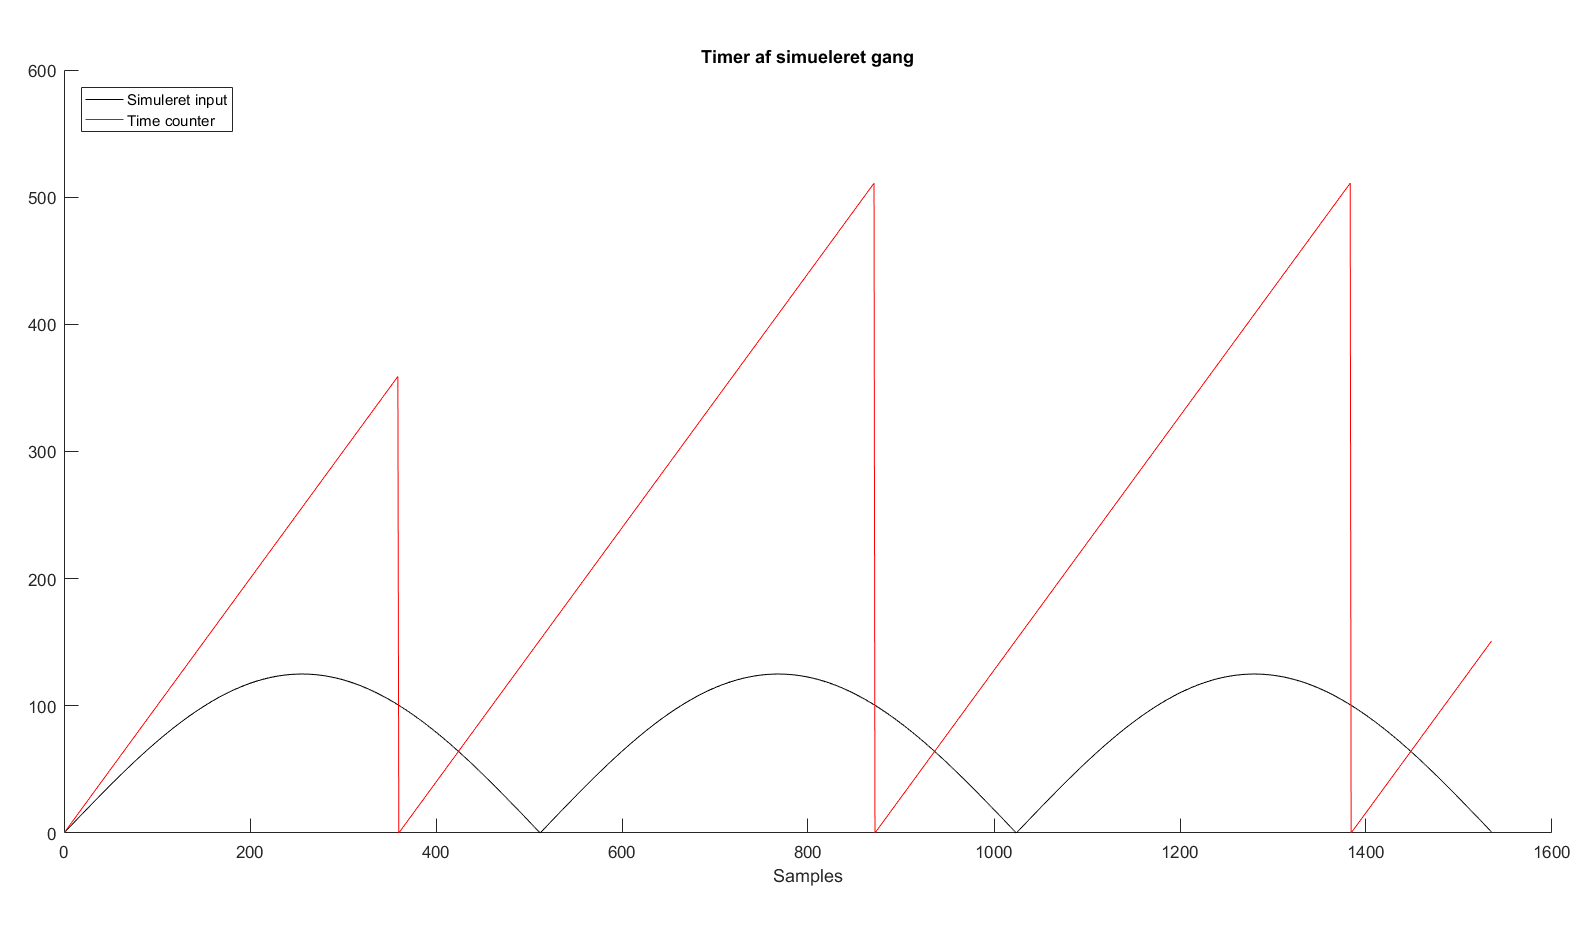
\includegraphics[width=.7\textwidth]{figures/cDesign/test_timecount_gang.png}
	\caption{På figuren ses algoritmen for gang, løb og ingen aktivitet vedrørende time counteren. Denne tæller op, indtil en sample har passeret under tærskelværdien, hvorefter den nulstilles. Den sorte kurve illustrerer det simulerede gangsignal, og den røde kurve er time counteren for algoritmen.}
	\label{fig:testgraf_timecounter}
\end{figure}\vspace{-0.25cm}
Algoritmens time counter starter, når signalet bliver indsendt og nulstilles efter en sample går under tærskelværdien. Heraf kan det ses, at varigheden fra en sample er gået over og under en tærskelværdi til, at en sample igen er gået over og under en tærskelværdi er 512~samples. En af algoritmens funktioner er at frasortere det første detekterede peak og dermed nulstille time counter værdien samt peak værdien. Det testes yderligere, om den første peak tælles med i videresendt data. I \tabref{tab:test_res_timecount} ses der, at selvom den første peak visualiseres i \figref{fig:testgraf_timecounter}, medregnes den ikke i de endelige værdier. Disse værdier fås ved hjælp af programmet Realterm, som visualiserer data fra MCUen.
\begin{table}[H]
	\centering
	\begin{tabular}{ccc}
		\hline
		\rowcolor[HTML]{C0C0C0} 
		Værdi videresendt & Forventet værdi [samples] & Modtaget værdi [samples] \\ \hline
		Time counter & $\emptyset$ - 512 - 512 & $\emptyset$ - 512 - 512 \\ \hline
	\end{tabular}
	\caption{I tabellen ses resultaterne for testen af algoritmens time counter. $\emptyset$ indikerer, at der ikke er modtaget en værdi.}
	\label{tab:test_res_timecount}
\end{table}\vspace{-0.25cm}
Algoritmen bliver testet på tre halvbølger. Det forventede resultat at varigheden af første peak bliver ikke medregnet og videresendt, som et resultat. Algoritmens timer counter fungerer som forventet, og videresender kun det forventede resultat uden afvigelse. Denne del af algoritmen accepteres og er klar til implementering i det samlede system.

I anden test af algoritmen tjekkes der for, om algoritmen giver korrekt værdi for detektering af den maksimale peak. Denne er designet således, at algoritmen ikke skal registre det første peak i et signal, som første test påviste. På \figref{fig:test_peak_gang} ses resultatet af testen.
\begin{figure}[H]
	\centering
	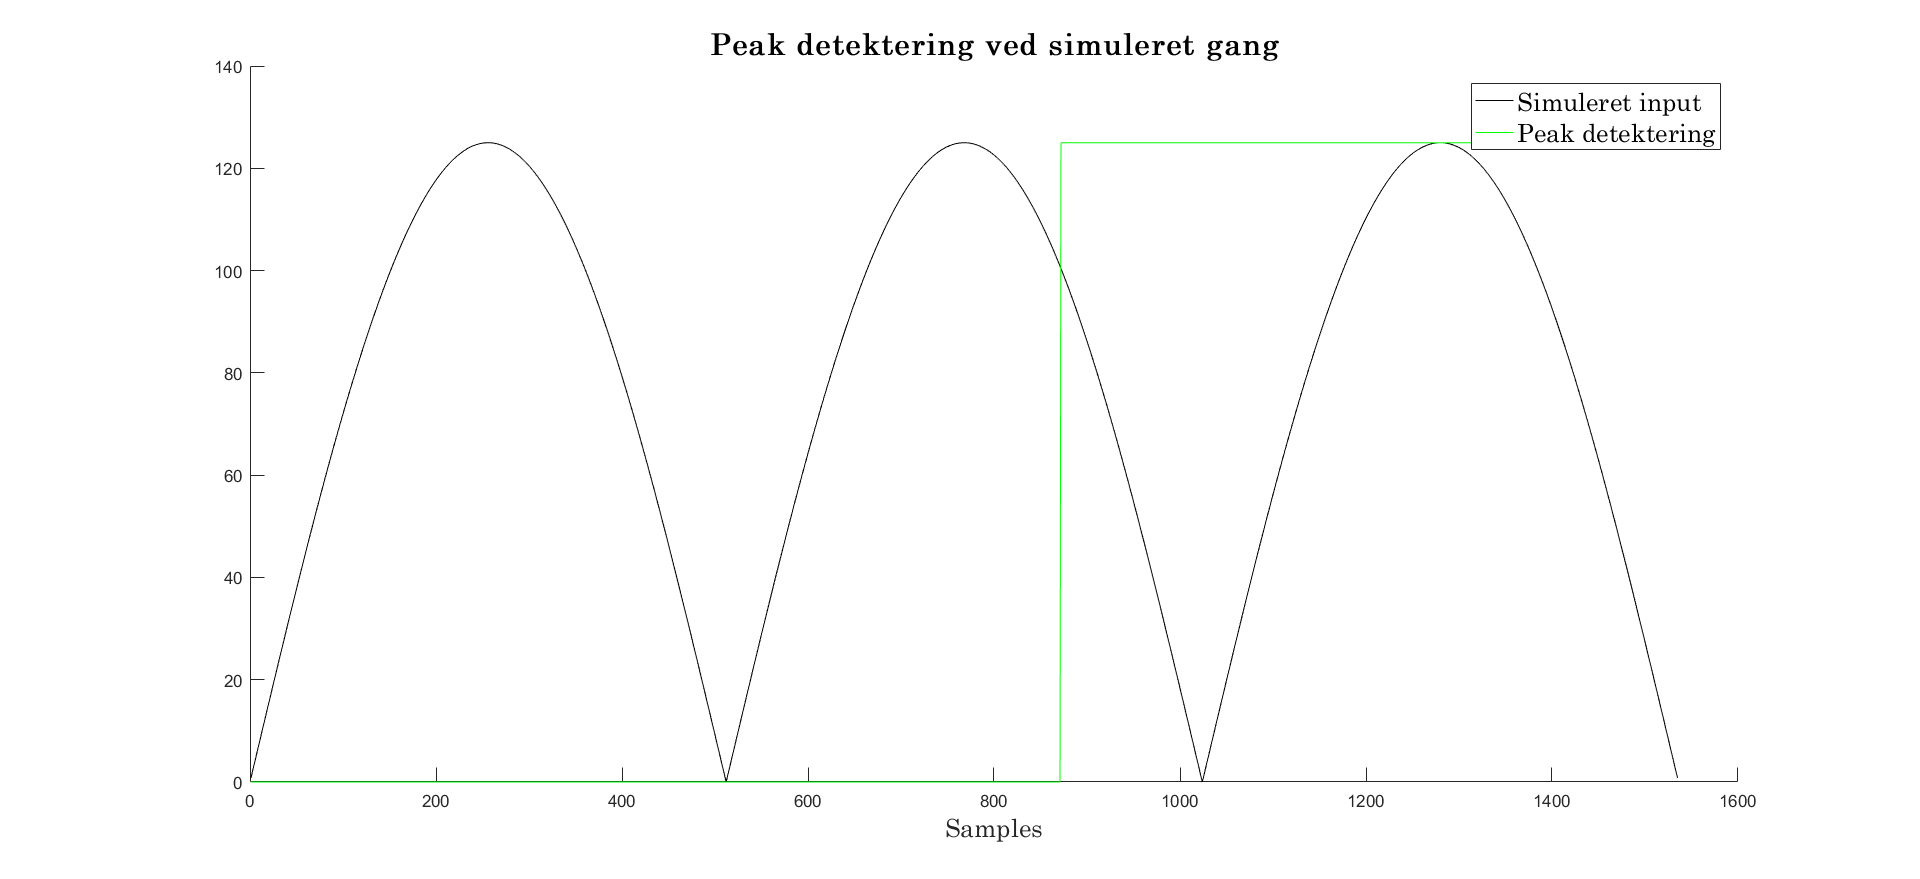
\includegraphics[width=.7\textwidth]{figures/cDesign/test_peak_gang.png}
	\caption{På figuren ses algoritmens funktion til at detektere værdien for det maksimale peak af et simuleret gangsignal. Den sorte kurve er det simulerede signal, og den røde kurve viser algoritmens funktion til detektering af peakværdier.}
	\label{fig:test_peak_gang}
\end{figure}\vspace{-0.25cm}
Det ses på \figref{fig:test_peak_gang}, at den første peak ikke detekteres, hvilket er grundet algoritmens design. Herefter findes værdien for det andet maksimale peak, når signalet er gået under tærskelværdien på 50. Da tredje maksimale peak har samme værdi som anden maksimale peak, forbliver den røde kurve på samme værdi.

Algoritmens detektering af peak starter, når en sample overskrider en bestemt tærskelværdi, hvilket ikke fremgår tydeligt på \figref{fig:test_peak_gang}. Algoritmen finder det maksimale peak, når en sample er under tærskelværdien, hvilket ses ud fra den røde graf. Hvis det første peak detekteres, sættes værdien til nul, således den ikke tælles med. På \figref{fig:test_peak_gang} kan det ses, at når signalet går under tærskelværdien anden gang, bliver peaket registreret. Den egentlige test vedrørende algoritmens detektering af peaks består dermed i at undersøge hvilke data, der videresendes som resultat, efter et simuleret input er kørt igennem algoritmen. Resultatet heraf ses i \tabref{tab:test_res_peak}, som fås ved hjælp af programmet Realterm, som visualiserer data fra MCUen.
\begin{table}[H]
	\centering
	\begin{tabular}{ccc}
		\hline
		\rowcolor[HTML]{C0C0C0} 
		Værdi videresendt & Forventet output [amplitude] & Output [amplitude] \\ \hline
		Peak detektering & $\emptyset$ - 100 - 100 & $\emptyset$ - 100 - 100 \\ \hline
	\end{tabular}
	\caption{I tabellen ses resultaterne for testen af algoritmens peak detektering. $\emptyset$ indikerer at der ikke er modtaget en værdi.}
	\label{tab:test_res_peak}
\end{table}\vspace{-0.25cm}
Algoritmen er blevet testet på tre halvbølger, og dermed er det forventede resultat, at peakværdien af det første peak ikke bliver medregnet og videresendt som et resultat. Algoritmens peak detektering fungerer dermed som forventet og videresender amplituderne uden afvigelse.

Algoritmen for løb bliver ligeledes testet med hensyn til funktionaliteten af time counter og peak detektering. Ved denne test bliver der indsendt et absolut sinussignal med en højere amplitude, som overskrider tærskelværdien vedrørende detektering af løb. Resultaterne af disse test medfører resultater af samme nøjagtighed, som ved detektering af gang. Algoritmen fungerer efter hensigten til detektering af gang og løb.

Algoritmen bør altså undersøge, hvorvidt data fra accelerometret klassificeres som ingen aktivitet, gang eller løb ved hjælp af tærskelværdier. I testen heraf indsendes et simuleret signal, som først overskrider tærskelværdierne for gang på 50. Herefter forekommer en periode på tre~sekunder, hvor hverken gang eller løbs tærskelværdi overskrides, hvorfor time counteren vil nulstille efter tre~sekunder uden overskridelse af nogen tærskelværdier. Afslutningsvis indsendes værdier, som overskrider tærskelværdierne vedrørende løb på 400. Herigennem bliver både time count og detektering af peaks testet, hvilket fremgår i \figref{fig:test_inaktiv_time} og \figref{fig:test_inaktiv_peak}. 
\begin{figure}[H]
	\centering
	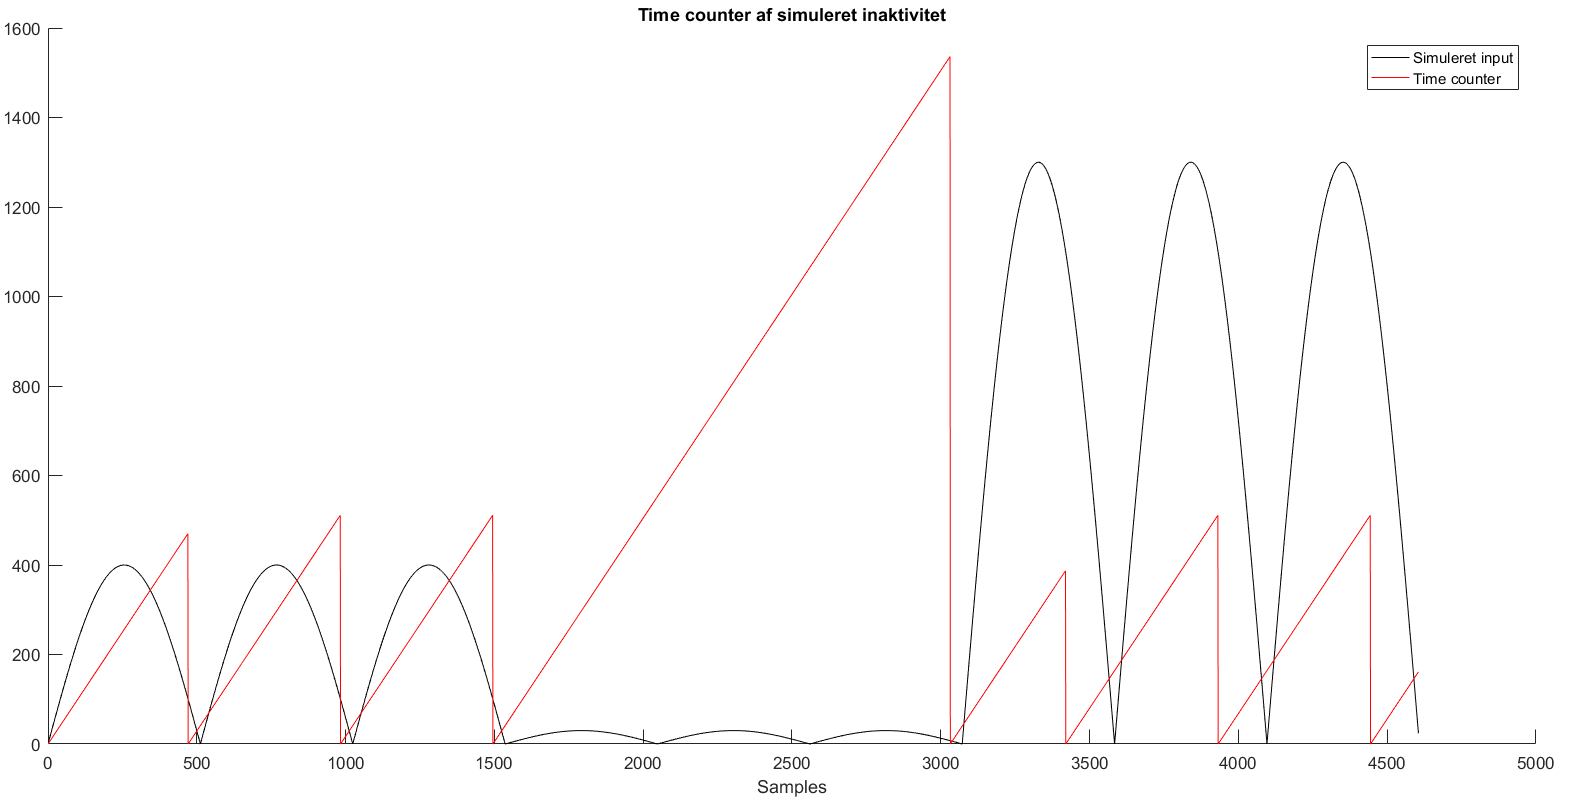
\includegraphics[scale=0.27]{figures/cDesign/test_timecount_inaktiv.png}
	\caption{På figuren ses algoritmens time counter, som ved detektering på et simuleret gang-, inaktiv- og løbesignal. Den sorte kurve er det simulerede signal, og den røde kurve viser algoritmens time counter af samples.}
	\label{fig:test_inaktiv_time}
\end{figure}\vspace{-0.25cm}
Der ses i midten af \figref{fig:test_inaktiv_time}, at time counteren nulstilles efter tre~sekunder selvom inden tærskelværdier er overskredet. Det er derfor fordelagtigt at smide værdien ud for første detekterede maksimale peak herefter.
\begin{figure}[H]
	\centering
	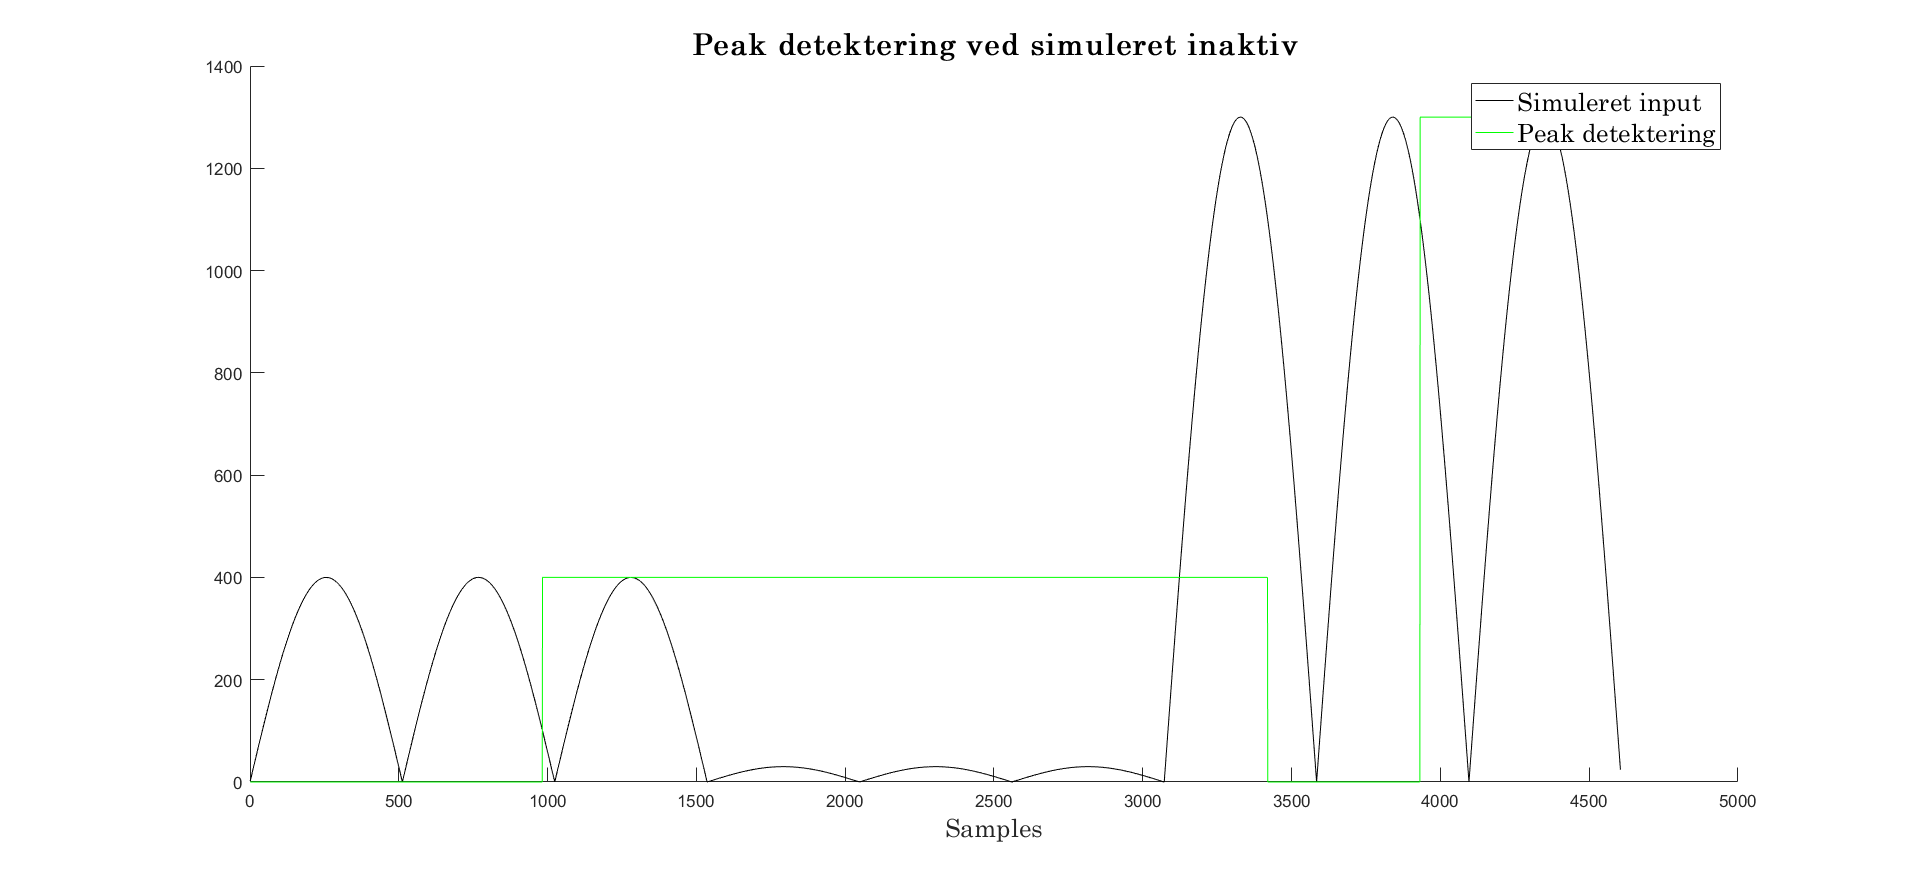
\includegraphics[width=.7\textwidth]{figures/cDesign/test_peak_inaktiv.png}
	\caption{På figuren ses algoritmens detektering af peaks på et simuleret signal. Den sorte kurve er det simulerede signal, og den røde kurve er detektering af peaks.}
	\label{fig:test_inaktiv_peak}
\end{figure}\vspace{-0.25cm}
Resultaterne vedrørende time count på \figref{fig:test_inaktiv_time} viser, at i perioden uden nogen aktivitet nulstilles time counteren hvert tredje sekund, hvis en sample ikke har været over og under en tærskelværdi. Resultaterne vedrørende detektering af peak på \figref{fig:test_inaktiv_peak} viser, at første værdi tilhørende det første peak samt det første peak efterfulgt fra ingen aktivitet frasorteres. For at klassificere hvorvidt algoritmen omhandlende detektering af ingen aktivitet fungerer efter hensigten, undersøges data, der bliver videresendt som et resultat af perioder uden aktivitet. I tilfælde med et signalinput som ovenstående bør det første peak frasorteres efterfulgt af to værdier. Resultatet fra denne test fremgår i \tabref{tab:test_inaktiv}.
\begin{table}[H]
	\centering
	\begin{tabular}{ccc}
		\hline
		\rowcolor[HTML]{C0C0C0} 
		Værdi videresendt & Forventet værdi & Modtaget værdi \\ \hline
		\begin{tabular}[c]{@{}c@{}}Time counter \\ {[}samples{]}\end{tabular} & $\emptyset$ - 512 - 512 - $\emptyset$ - 512 - 512 & $\emptyset$ - 512 - 512 - $\emptyset$ - 512 - 512 \\ \hline
		\begin{tabular}[c]{@{}c@{}}Peak detektering \\ {[}amplitude{]}\end{tabular} &     $\emptyset$ - 200 - 200 - $\emptyset$ - 600 - 600     &    $\emptyset$ - 200 - 200 - $\emptyset$ - 600 - 600 \\ \hline
	\end{tabular}
	\caption{I tabellen ses resultaterne for testen af algoritmens time counter og peak detektering. $\emptyset$ indikerer at der ikke er modtaget en værdi.}
	\label{tab:test_inaktiv}
\end{table}\vspace{-0.25cm}
Algoritmen er testet på et simuleret signal, som illustrer en periode uden aktivitet omringet af to perioder med henholdsvis gang og løb. Det forventede resultat for både time count værdien og peakværdien er, at det første peak frasorteres, og første peak efter en periode uden aktivitet frasorteres. Dermed forventes det, at det videresendte data er time count på 512, og amplituder som afspejler signalets udformning på 200 og 600. Resultatet af det data, som bliver modtaget, er som forventet uden afvigelse, og det antages derfor at algoritmens funktion vedrørende detektering af perioder uden aktivitet fungerer efter hensigten. Denne del af algoritmen accepteres og er klar til implementering i det samlede system.